\section{Avaliação do Memora}
\label{sec:avaliacao}

A avaliação investigou a experiência de uso do Memora, com atenção à configuração, ao acompanhamento dos acessos e à interpretação das informações da cache. Foram realizadas sete entrevistas individuais com estudantes, compondo um único ciclo de avaliação. O procedimento reuniu tarefas, observação da interação, perguntas abertas e uma avaliação rápida da experiência de uso. Esta seção apresenta a preparação, a execução, os resultados e os ajustes decorrentes dos achados.

\subsection{Metodologia da avaliação}
\label{sec:plano-avaliacao}

A organização em preparação, execução e análise tomou como referência o estudo do MedSimples de \citeonline{macedo2025medsimples} e os procedimentos de avaliação de IHC descritos por \citeonline{barbosa2010ihc}. Na preparação, foram definidos o perfil dos estudantes, as tarefas, as fichas de parâmetros e as perguntas após o uso. O roteiro e as fichas estão no Apêndice~\ref{ap:roteiro-memora}. A aplicação também oferece um manual visual, reproduzido no Apêndice~\ref{ap:manual-visual}.

As tarefas abrangeram quatro objetivos:
\begin{enumerate}
\item[\textbf{T1.}] Carregar o exemplo, ajustar a sequência conforme a ficha A, conferir os parâmetros e localizar uma explicação de um campo.
\item[\textbf{T2.}] Acompanhar a simulação, usar os controles, localizar uma substituição no histórico, examinar o antes/depois e identificar os totais e a conclusão.
\item[\textbf{T3.}] Retornar à configuração, utilizar a ficha B e observar as diferenças ao mudar o mapeamento.
\item[\textbf{T4.}] Alterar a memória principal conforme a ficha C e observar o efeito na divisão do endereço.
\end{enumerate}

Na execução, cada estudante utilizou o Memora individualmente, enquanto o entrevistador registrava tempos, ações, dificuldades, intervenções e comentários. Após as tarefas, foram feitas perguntas sobre o que ajudou ou dificultou o uso, as mudanças percebidas entre configurações e as melhorias desejadas. A avaliação rápida considerou quatro critérios: facilidade para começar e usar os controles (C1), clareza das informações (C2), apoio à visualização dos mapeamentos e parâmetros (C3) e satisfação (C4).

Na análise, os registros foram reunidos por participante e tarefa. Foram examinados os episódios de uso e as respostas abertas, mantendo as alternativas da avaliação rápida conforme anotadas. As apreciações sobre o Beto foram retrospectivas, a partir da experiência anterior dos estudantes; as tarefas observadas foram executadas no Memora.

\subsection{Participantes e execução das sessões}

Participaram sete estudantes de Engenharia de Computação selecionados por conveniência, todos em seu primeiro contato com o Memora. Seis cursavam o quinto período e um estava em etapa mais avançada do curso. Cinco já haviam utilizado o Beto. A Tabela~\ref{tab:perfil-participantes} apresenta essa experiência, preservando o anonimato por meio dos códigos P01--P07.

\begin{table}[!htbp]\centering
\caption{Experiência prévia dos participantes com o Beto.}\label{tab:perfil-participantes}
\small
\begin{tabular}{@{}P{1.6cm}P{12.3cm}@{}}
\toprule\textbf{Código} & \textbf{Experiência prévia}\\\midrule
P01 & Uso no semestre anterior.\\
P02 & Uso no semestre anterior.\\
P03 & Sem uso prévio.\\
P04 & Uso em Laboratório de Arquitetura e Organização de Computadores II (LAOC II).\\
P05 & Uso em disciplina de AOC e pouco contato em laboratório.\\
P06 & Sem uso prévio.\\
P07 & Uso em LAOC II.\\
\bottomrule
\end{tabular}
\par\footnotesize Fonte: fichas anonimizadas. Todos utilizaram o Memora pela primeira vez.
\end{table}

As sessões seguiram os quatro objetivos do roteiro, com esclarecimentos e intervenções quando surgiram dúvidas. Em T2, P04 e P05 receberam orientação para desativar as etapas detalhadas. Em T3, P06 recebeu indicação sobre esse modo e sobre um acesso a consultar. P07 acompanhou o segundo cenário sem o passo a passo e recebeu indicação do acesso a examinar em T2. Também ocorreram perguntas de confirmação e orientações sobre as fichas. Essas condições são consideradas na interpretação dos resultados.

\subsection{Principais resultados}

\subsubsection{Execução das tarefas}

A Tabela~\ref{tab:tempos-entrevista} registra os tempos anotados e a Figura~\ref{fig:tempos-tarefas} apresenta os sete participantes em uma única série de sessões. Os subtotais abrangem as tarefas com duração registrada, sem incluir a entrevista após o uso. T4 de P01 ficou sem tempo anotado. Em T4 de P02, há um tempo registrado, mas a execução do objetivo está parcialmente documentada. Em T1, P01 avançou à simulação sob um enunciado impreciso.

\begin{table}[!htbp]\centering
\caption{Tempos anotados nas tarefas, em minutos e segundos.}\label{tab:tempos-entrevista}
\small
\begin{tabular}{@{}lccccc@{}}
\toprule\textbf{Código} & \textbf{T1} & \textbf{T2} & \textbf{T3} & \textbf{T4} & \textbf{Subtotal}\\\midrule
P01 & 1:34 & 1:30 & 1:00 & SR & 4:04$^{a}$\\
P02 & 1:00 & 1:00 & 0:30 & 1:00$^{b}$ & 3:30$^{b}$\\
P03 & 1:57 & 3:43 & 2:00 & 1:20 & 9:00\\
P04 & 1:00 & 2:30 & 1:00 & 1:00 & 5:30\\
P05 & 0:50 & 1:30 & 1:30 & 1:10 & 5:00\\
P06 & 0:50 & 3:00 & 1:50 & 0:30 & 6:10\\
P07 & 1:42 & 2:43 & 1:20 & 1:36 & 7:21\\
\bottomrule
\end{tabular}
\par\footnotesize Fonte: fichas das sessões. SR: sem registro. $^{a}$ Soma de T1--T3. $^{b}$ T4 parcialmente documentada.
\end{table}

\begin{figure}[!htbp]\centering
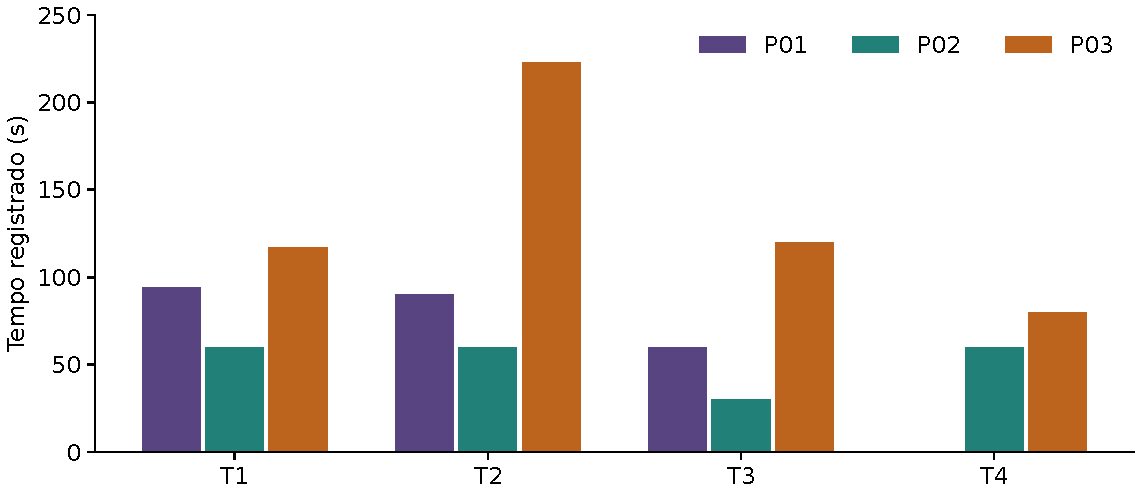
\includegraphics[width=\linewidth]{figuras/tempos-tarefas.pdf}
\caption{Tempos registrados por tarefa e participante.}\label{fig:tempos-tarefas}
\par\footnotesize Fonte: elaboração própria com base nas fichas P01--P07. Os tempos dependem da condução e da ajuda recebida em cada sessão.
\end{figure}

Na configuração, os registros descrevem edição dos parâmetros e da sequência, além de consulta às explicações. P07 destacou a correção durante o preenchimento e comentou: ``Ele te corrige em tempo real né digamos assim''. Nos testes com valor zero solicitados pelo moderador a P05 e P07, os participantes observaram o retorno da validação. A apresentação próxima aos campos permitiu discutir a relação entre entrada e restrição antes da execução.

No acompanhamento dos acessos, P01 valorizou espontaneamente a descrição dos eventos. P02 usou reprodução, pausa, velocidade e avanço, mas perguntou pela diferença entre Parar e Pausar. P02 e P03 não reconheceram inicialmente o marcador circular do histórico como uma ação. Após receber a indicação, P02 comentou: ``se você não falar eu não teria visto isso aí''. P03 afirmou: ``Não sabia que era um botão''. Esses episódios apontaram um problema de identificação do controle de revisão.

P04 localizou uma substituição e confirmou ter consultado a comparação e os totais. P05 abriu Analisar por iniciativa própria e verbalizou dois acertos, seis faltas, taxa de 25\% e progresso finalizado. P06 utilizou a descrição do evento para explicar uma falta, mas perguntou como retornar ao estado atual da simulação. P07 reconheceu o botão de análise e consultou o antes/depois após a indicação de um acesso. Os registros desses episódios variam quanto ao detalhamento dos blocos e dos totais identificados.

Ao mudar o mapeamento, os estudantes comentaram a organização e a disponibilidade dos campos. P05 distinguiu a explicação de LRU do uso de uma via livre, sem remoção. P06 percebeu diferenças entre as fichas com orientação sobre a consulta ao histórico. Na alteração da memória principal, P03 percebeu uma mudança visual e precisou de direcionamento para identificar seu significado; P04--P07 também alteraram a quantidade de palavras e comentaram mudanças na tela. Esses resultados mostram como a representação foi utilizada, sem permitir comparar a autonomia apenas pelos tempos.

\subsubsection{Entrevista após o uso}

As respostas abertas indicaram apreciação pela organização, pelas descrições dos acessos e pela ajuda. P01 comentou que o Memora ``é bem intuitivo e melhor que o Beto'', segundo anotação literal confirmada pelo entrevistador. Essa comparação expressa a lembrança de uma experiência anterior. P04 valorizou o histórico, os blocos e a comparação, sem indicar uma melhoria prioritária.

P05 destacou a possibilidade de configurar exercícios e revisar o conteúdo, além do manual, do exemplo pronto, do Glossário e da Ajuda rápida. Considerou, porém, rápida a reprodução: ``eu acho que essa velocidade podia ser menor tipo assim no dois ele ainda é muito rápido''. Sugeriu também a edição dos endereços em blocos interativos, para reduzir erros de digitação.

P06 valorizou a separação entre memória principal e cache e a explicação por acesso. Ao discutir o retorno da comparação, comentou: ``Talvez dá pra deixar esse botão mais mais aparente''. Também sugeriu explicações breves sobre mapeamentos e LRU. P07 destacou o alinhamento de linha e via e associou a ferramenta à revisão do conteúdo: ``só com esse simulador eu consigo relembrar o conteúdo sabe''.

Os trechos de P02--P07 provêm das transcrições fornecidas. A análise das perguntas abertas preservou a relação entre participante e pergunta e considerou que uma resposta poderia conter mais de um tema. As sugestões mais específicas se concentraram na descoberta do histórico, no retorno ao estado atual, no ritmo da reprodução e no apoio à configuração.

\subsubsection{Avaliação rápida da experiência de uso}

A escala oferecia C (atende completamente), P (atende parcialmente), N (não atende) e X (não conseguiu avaliar). A matriz da Tabela~\ref{tab:matriz-rapida} apresenta as alternativas efetivamente registradas. SR identifica ausência de código, preservando os relatos qualitativos sem convertê-los em alternativas da escala.

\begin{table}[!htbp]\centering
\caption{Alternativas registradas na avaliação rápida dos sete participantes.}\label{tab:matriz-rapida}
\begin{tabular}{lcccc}
\toprule\textbf{Participante} & \textbf{C1} & \textbf{C2} & \textbf{C3} & \textbf{C4}\\\midrule
P01 & C & C & C & C\\
P02 & SR & SR & SR & SR\\
P03 & SR & SR & SR & SR\\
P04 & C & C & C & C\\
P05 & C & C & C & C\\
P06 & C & C & C & C\\
P07 & C & C & C & SR$^{a}$\\
\bottomrule
\end{tabular}
\par\footnotesize C1: controles; C2: clareza; C3: mapeamentos e parâmetros; C4: satisfação. SR: sem código registrado. $^{a}$ P07 respondeu ``Muito positiva'' em texto. Fonte: fichas anonimizadas.
\end{table}

P01 e P04--P06 possuem C nos quatro critérios; P07 possui C em C1--C3. Os registros de P02 e P03 são qualitativos: descrevem apreciações favoráveis e ressalvas sobre a descoberta da revisão, os comandos e a organização. A satisfação de P07 foi registrada como ``Muito positiva'', sem alternativa. As marcações de P04 em C3 e de P05 em C2/C4 se apoiam nas anotações consolidadas.

A Figura~\ref{fig:avaliacao-rapida} utiliza sete participantes como base em cada critério. Em C1--C3, houve cinco respostas C (71,4\%) e dois registros sem código (28,6\%). Em C4, houve quatro respostas C (57,1\%) e três sem código (42,9\%). Não houve marcações P, N ou X. A distribuição apresenta simultaneamente as respostas obtidas e a cobertura dos registros da escala.

\begin{figure}[!htbp]\centering
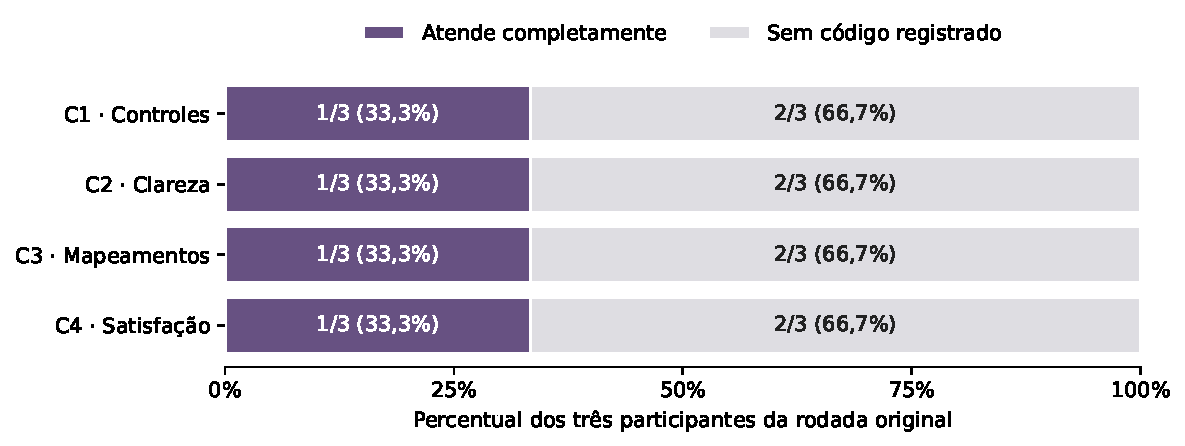
\includegraphics[width=\linewidth]{figuras/avaliacao-rapida.pdf}
\caption{Distribuição das respostas e cobertura da avaliação rápida.}\label{fig:avaliacao-rapida}
\par\footnotesize Fonte: elaboração própria; base de sete participantes em cada critério.
\end{figure}

\subsection{Ajustes decorrentes da avaliação}

Os episódios observados orientaram refinamentos de interface. A Tabela~\ref{tab:achados-ajustes} relaciona os problemas e as sugestões às alterações implementadas ao longo do desenvolvimento. A consulta aos estados anteriores passou a utilizar uma ação textual explícita, e o retorno à execução foi aproximado da própria cache. As sugestões de ritmo, edição e ajuda também foram incorporadas à evolução da aplicação.

\begin{longtable}{@{}P{5.6cm}P{8.2cm}@{}}
\caption{Observações de uso e alterações realizadas na interface.}\label{tab:achados-ajustes}\\
\toprule\textbf{Observação ou sugestão} & \textbf{Alteração implementada}\\\midrule\endfirsthead
\toprule\textbf{Observação ou sugestão} & \textbf{Alteração implementada}\\\midrule\endhead
P02 e P03 não reconheceram a ação no marcador circular do histórico. & Introdução de botão textual de revisão, posteriormente denominado Analisar e associado ao número do acesso.\\\midrule
P02 questionou a diferença entre Parar e Pausar. & Simplificação dos comandos e dos estados de reprodução, com retirada do controle redundante.\\\midrule
P06 pediu ajuda para retornar ao estado atual. & Posicionamento de Voltar ao estado atual no cabeçalho de Memória cache.\\\midrule
P05 considerou rápida a velocidade 2. & Ampliação do controle para ritmos mais lentos, incluindo 0,25 passo ou acesso por segundo, conforme o modo.\\\midrule
P05 sugeriu editar endereços em blocos. & Inclusão de editor opcional por endereço, com validação e possibilidade de aplicar ou descartar a edição.\\\midrule
P06 sugeriu explicações breves dos mapeamentos. & Inclusão de ajuda próxima à seleção do mapeamento.\\
\bottomrule
\end{longtable}

A Figura~\ref{fig:memora-revisao} ilustra a comparação e o retorno no cabeçalho da cache. As capturas deste artigo e do manual apresentam cenários ilustrativos da evolução da aplicação; não documentam as telas de cada entrevista. Os ajustes implementados após a observação correspondente ainda precisam ser reavaliados com usuários para verificar se resolvem as dificuldades identificadas.

\begin{figure}[!htbp]\centering
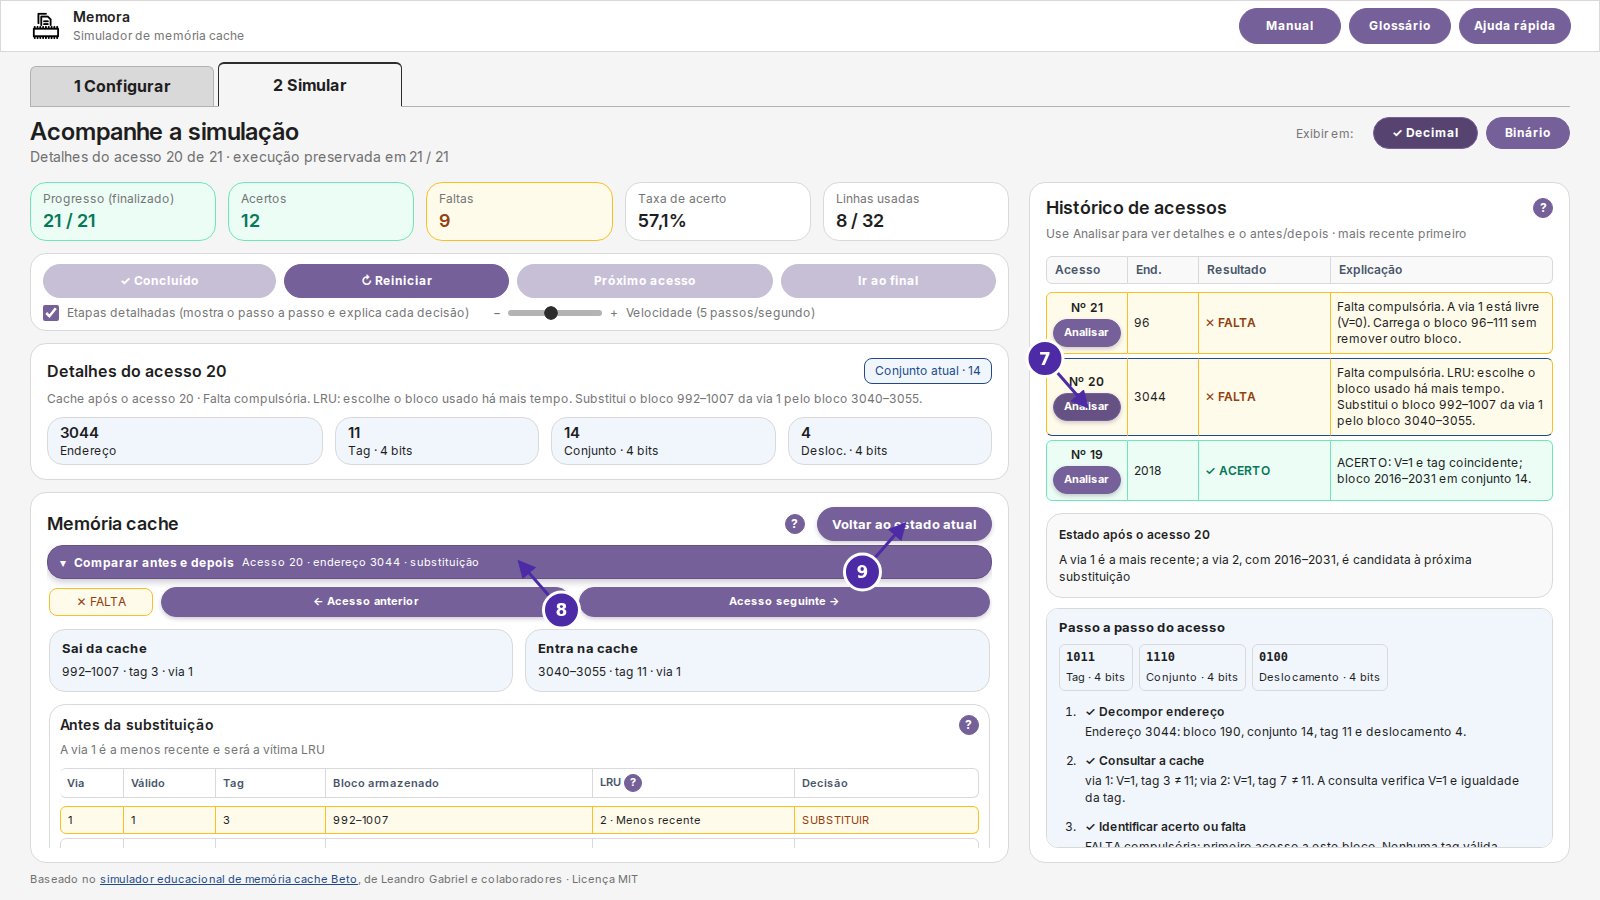
\includegraphics[width=\linewidth,height=.39\textheight,keepaspectratio]{figuras/manual/comparacao.png}
\caption{Comparação antes/depois de um acesso e retorno ao estado atual.}\label{fig:memora-revisao}
\par\footnotesize Fonte: captura própria da aplicação; cenário ilustrativo de substituição com LRU.
\end{figure}
